\documentclass[a4paper]{paper}

\usepackage{fullpage}
\usepackage[utf8]{inputenc}
\usepackage[T1]{fontenc}
\usepackage{amsthm}

\usepackage{color}
\newcommand{\xcol}{blue}
\newcommand{\ycol}{red}

\usepackage{tikz}

\newcommand{\nomFormat}{Fodaly}
\newtheorem{definition}{Definition}


\title{\nomFormat{}~: un format textuel de description (d'arènes) de labyrinthes}
%\author{L. Jezequel}
%\date{Le 23 mai 2016}

\author{\textrm{Projet} \textsf{Tremplin en DUT informatique}\\
\textrm{IUT de Nantes - Année 2016--2017}}



\begin{document}

\maketitle

\section{Grilles, murs, arènes, labyrinthes}

On considère des \emph{grilles} constituées de cases, auxquelles on associe des coordonnées : une abscisse ($x$) et une ordonnée ($y$).
La figure~\ref{fig:grille} (gauche) donne un exemple d'une telle grille.
La case repérée en vert a pour abscisse $2$ et pour ordonnée $1$, on dira donc que c'est la case de coordonnées $(2, 1)$. Notons qu'on commence la numérotation par 0.

On peut placer des \emph{murs} horizontaux et verticaux le long des cases d'une telle grille.
Sur la figure~\ref{fig:grille} (milieu gauche par exemple), les murs sont représentés par des traits noirs épais.

\begin{definition}{(arène)}
On appelle une \emph{arène} une grille entièrement entourée de murs.
\end{definition}

Sur la figure~\ref{fig:grille} (milieu droit) une telle arène est représentée.

Un point de départ est une coordonnée $(x,y)$ donnée sur une grille. 
De m\^eme un point d'arrivée est une coordonnée $(x,y)$ donnée sur une grille, et telle que cette coordonnée représente une case en bordure de la grille. 

\begin{definition}{(\emph{labyrinthe})}
Un labyrinthe est une arène, avec  un point de départ (D) et un point d'arrivée (A), et telle qu'il est possible en partant du point de départ, d'atteindre le point d'arrivée en se déplaçant entre cases adjacentes sans jamais couper un mur.
%En ajoutant un point de départ et un point d'arrivée à une arène on obtient un \emph{labyrinthe}, à condition qu'il soit possible d'atteindre l'arrivée depuis le départ en se déplacent entre cases adjacentes sans jamais couper un mur.
\end{definition}

Sur la figure~\ref{fig:grille} (droite) un labyrinthe est représenté.
Le départ est noté D et l'arrivée A.


\begin{figure}[htbp]
  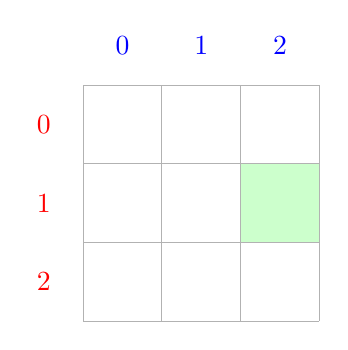
\begin{tikzpicture}

    \node[\xcol] (x1) at (0.5, 0.5) {0};
    \node[\xcol] (x2) at (1.5, 0.5) {1};
    \node[\xcol] (x3) at (2.5, 0.5) {2};

    \node[\ycol] (y1) at (-0.5, -0.5) {0};
    \node[\ycol] (y2) at (-0.5, -1.5) {1};
    \node[\ycol] (y3) at (-0.5, -2.5) {2};

    % exemple de case
    \draw[fill=green!20, draw=none] (2, -1) rectangle (3, -2);
    
    \draw[draw=black!30] (0, 0) -- (3, 0);
    \draw[draw=black!30] (0, -1) -- (3, -1);
    \draw[draw=black!30] (0, -2) -- (3, -2);
    \draw[draw=black!30] (0, -3) -- (3, -3);
    \draw[draw=black!30] (0, 0) -- (0, -3);
    \draw[draw=black!30] (1, 0) -- (1, -3);
    \draw[draw=black!30] (2, 0) -- (2, -3);
    \draw[draw=black!30] (3, 0) -- (3, -3);
    
  \end{tikzpicture}
  \hfill
  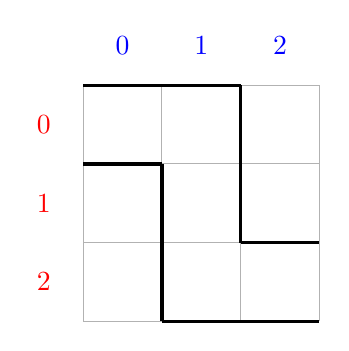
\begin{tikzpicture}

    \node[\xcol] (x1) at (0.5, 0.5) {0};
    \node[\xcol] (x2) at (1.5, 0.5) {1};
    \node[\xcol] (x3) at (2.5, 0.5) {2};

    \node[\ycol] (y1) at (-0.5, -0.5) {0};
    \node[\ycol] (y2) at (-0.5, -1.5) {1};
    \node[\ycol] (y3) at (-0.5, -2.5) {2};
    
    \draw[draw=black!30] (0, 0) -- (3, 0);
    \draw[draw=black!30] (0, -1) -- (3, -1);
    \draw[draw=black!30] (0, -2) -- (3, -2);
    \draw[draw=black!30] (0, -3) -- (3, -3);
    \draw[draw=black!30] (0, 0) -- (0, -3);
    \draw[draw=black!30] (1, 0) -- (1, -3);
    \draw[draw=black!30] (2, 0) -- (2, -3);
    \draw[draw=black!30] (3, 0) -- (3, -3);

    \draw[draw=black, very thick] (0, 0) -- (2, 0);
    \draw[draw=black, very thick] (0, -1) -- (1, -1);
    \draw[draw=black, very thick] (1, -1) -- (1, -3);
    \draw[draw=black, very thick] (2, 0) -- (2, -2);
    \draw[draw=black, very thick] (1, -3) -- (3, -3);
    \draw[draw=black, very thick] (2, -2) -- (3, -2);
    
  \end{tikzpicture}
  \hfill
  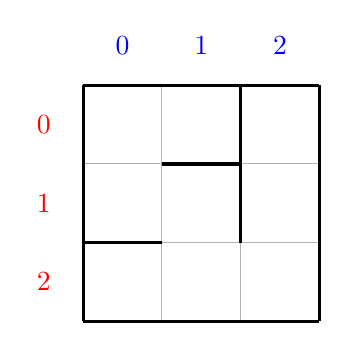
\begin{tikzpicture}

    \node[\xcol] (x1) at (0.5, 0.5) {0};
    \node[\xcol] (x2) at (1.5, 0.5) {1};
    \node[\xcol] (x3) at (2.5, 0.5) {2};

    \node[\ycol] (y1) at (-0.5, -0.5) {0};
    \node[\ycol] (y2) at (-0.5, -1.5) {1};
    \node[\ycol] (y3) at (-0.5, -2.5) {2};
    
    \draw[draw=black!30] (0, 0) -- (3, 0);
    \draw[draw=black!30] (0, -1) -- (3, -1);
    \draw[draw=black!30] (0, -2) -- (3, -2);
    \draw[draw=black!30] (0, -3) -- (3, -3);
    \draw[draw=black!30] (0, 0) -- (0, -3);
    \draw[draw=black!30] (1, 0) -- (1, -3);
    \draw[draw=black!30] (2, 0) -- (2, -3);
    \draw[draw=black!30] (3, 0) -- (3, -3);

    \draw[draw=black, very thick] (0, 0) -- (3, 0);
    \draw[draw=black, very thick] (0, -3) -- (3, -3);
    \draw[draw=black, very thick] (0, 0) -- (0, -3);
    \draw[draw=black, very thick] (3, 0) -- (3, -3);
    \draw[draw=black, very thick] (2, 0) -- (2, -2);
    \draw[draw=black, very thick] (1, -1) -- (2, -1);    
    \draw[draw=black, very thick] (0, -2) -- (1, -2);    
    
  \end{tikzpicture}
  \hfill
  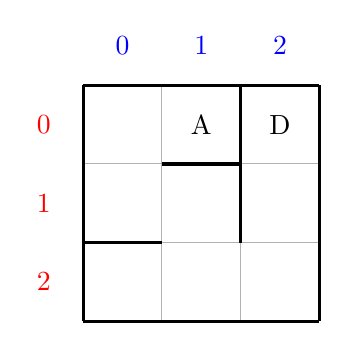
\begin{tikzpicture}
      
    \node[\xcol] (x1) at (0.5, 0.5) {0};
    \node[\xcol] (x2) at (1.5, 0.5) {1};
    \node[\xcol] (x3) at (2.5, 0.5) {2};

    \node[\ycol] (y1) at (-0.5, -0.5) {0};
    \node[\ycol] (y2) at (-0.5, -1.5) {1};
    \node[\ycol] (y3) at (-0.5, -2.5) {2};
    
    \draw[draw=black!30] (0, 0) -- (3, 0);
    \draw[draw=black!30] (0, -1) -- (3, -1);
    \draw[draw=black!30] (0, -2) -- (3, -2);
    \draw[draw=black!30] (0, -3) -- (3, -3);
    \draw[draw=black!30] (0, 0) -- (0, -3);
    \draw[draw=black!30] (1, 0) -- (1, -3);
    \draw[draw=black!30] (2, 0) -- (2, -3);
    \draw[draw=black!30] (3, 0) -- (3, -3);

    \draw[draw=black, very thick] (0, 0) -- (3, 0);
    \draw[draw=black, very thick] (0, -3) -- (3, -3);
    \draw[draw=black, very thick] (0, 0) -- (0, -3);
    \draw[draw=black, very thick] (3, 0) -- (3, -3);
    \draw[draw=black, very thick] (2, 0) -- (2, -2);
    \draw[draw=black, very thick] (1, -1) -- (2, -1);    
    \draw[draw=black, very thick] (0, -2) -- (1, -2);    

    \node (d) at (2.5, -0.5) {D};
    \node (a) at (1.5, -0.5) {A};
    
  \end{tikzpicture}
  \caption{Une grille, des murs sur une grille, une arène, un labyrinthe}\label{fig:grille}
\end{figure}

Le reste de ce document présente le format de fichier \nomFormat{}, permettant de décrire des arènes.

\section{Le format \nomFormat{}}

\subsection{Principe de base}

On remarque que des murs sur une grille peuvent être décrits ligne par ligne. 
Ici, chaque ligne d'une grille est représentée systématiquement par deux descriptions : \\
\textit{i)} l'indication de la présence ou l'absence d'un mur horizontal en haut de chaque case de la ligne ; \\
\textit{ii)} l'indication de la présence ou l'absence d'un mur vertical à gauche de chaque case de la ligne.

Par exemple on indique d'abord, pour chaque case d'ordonnée $0$ si elle a un mur horizontal en haut ou pas, puis pour chaque case d'ordonnée $0$ si elle a  un mur vertical à gauche ou pas.
Ainsi, pour l'exemple de la figure~\ref{fig:format1}, on indiquera \textit{i)} \verb|mur-pasmur-pasmur| et \textit{ii)} \verb|pasmur-pasmur-mur|.
%On peut ensuite indiquer, toujours pour chaque case d'ordonnée $0$ si elle a un mur vertical à gauche ou pas. Toujours sur le même exemple, on indiquera \verb|pasmur-pasmur-mur|.

Sur le même principe on passe à la ligne d'ordonnée $1$ (\verb|pasmur-mur-pasmur| puis \verb|mur-pasmur-mur|) et ensuite à la ligne d'ordonnée $2$ (\verb|mur-pasmur-pasmur| et enfin \verb|mur-pasmur-pasmur|).

Notez que si on a une grille de $n$ lignes, sa description fera $2 \times n$ lignes.

\begin{figure}[htbp]
  \centering
  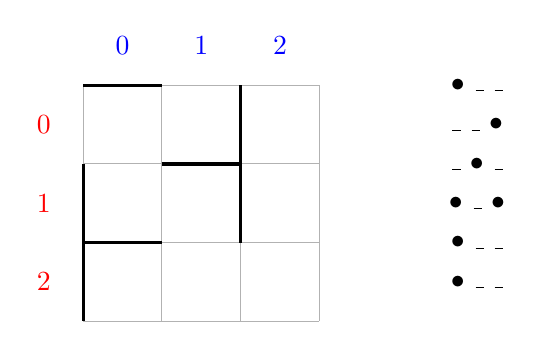
\begin{tikzpicture}

    \node[\xcol] (x1) at (0.5, 0.5) {0};
    \node[\xcol] (x2) at (1.5, 0.5) {1};
    \node[\xcol] (x3) at (2.5, 0.5) {2};

    \node[\ycol] (y1) at (-0.5, -0.5) {0};
    \node[\ycol] (y2) at (-0.5, -1.5) {1};
    \node[\ycol] (y3) at (-0.5, -2.5) {2};
    
    \draw[draw=black!30] (0, 0) -- (3, 0);
    \draw[draw=black!30] (0, -1) -- (3, -1);
    \draw[draw=black!30] (0, -2) -- (3, -2);
    \draw[draw=black!30] (0, -3) -- (3, -3);
    \draw[draw=black!30] (0, 0) -- (0, -3);
    \draw[draw=black!30] (1, 0) -- (1, -3);
    \draw[draw=black!30] (2, 0) -- (2, -3);
    \draw[draw=black!30] (3, 0) -- (3, -3);

    \draw[draw=black, very thick] (0, 0) -- (1, 0);
    \draw[draw=black, very thick] (0, -1) -- (0, -3);
    \draw[draw=black, very thick] (2, 0) -- (2, -2);
    \draw[draw=black, very thick] (1, -1) -- (2, -1);    
    \draw[draw=black, very thick] (0, -2) -- (1, -2);    
    
  \node at (5, 0) {$\bullet{}$ \_ \_};
  \node at (5, -0.5) {\_ \_ $\bullet{}$};
  \node at (5, -1) {\_ $\bullet{}$ \_};
  \node at (5, -1.5) {$\bullet{}$ \_ $\bullet{}$};
  \node at (5, -2) {$\bullet{}$ \_ \_};
  \node at (5, -2.5) {$\bullet{}$ \_ \_};
  \end{tikzpicture}  
  \caption{Encore des murs sur une grille}\label{fig:format1}
\end{figure}

\medskip
Pour réduire la taille de la représentation de l'arène on représentera chaque mur par un caractère visible différent de «~\_~» (dans l'exemple $\bullet{}$) et chaque absence de mur par le caractère «~\_~».
Ainsi, la grille de la figure~\ref{fig:format1} pourra être représentée par le texte à sa droite sur cette même figure. 

Ce texte décrivant la grille peut \^etre enregistré dans un fichier auquel on donnera un nom, pour le conserver, et pour pouvoir utiliser l'arène dans un programme.

Noter que le symbole $\bullet{}$ utilisé pour la présence d'un mur en haut ou à gauche d'une case de la grille, peut \^etre remplacé dans la description textuelle par \textbf{H} ou \textbf{G}. Par exemple la première ligne de la grille  de la figure~\ref{fig:format1} se décrit par  {H \_ \_} puis {\_ \_ G}.

\subsection{Le format complet}

En pratique, pour être certain qu'un fichier au format \nomFormat{} représente toujours une arène correcte, et pour éviter de devoir décrire tous les murs qui entourent cette arène, on s'autorisera à ne pas décrire les contours.
Ainsi, le texte de la figure~\ref{fig:format1} représentera plutôt l'arène donnée à la figure~\ref{fig:format2}.

De plus, si on saute une ligne dans la description d'une arène, ceci démarre la description d'une nouvelle colonne de l'arène.
Par exemple, la représentation donnée à la figure~\ref{fig:format2} décrit exactement la même arène que celle donnée à la figure~\ref{fig:format1}.

\begin{figure}[htbp]
  \centering
  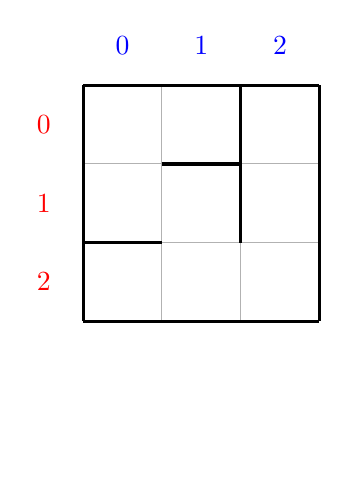
\begin{tikzpicture}

    \node[\xcol] (x1) at (0.5, 0.5) {0};
    \node[\xcol] (x2) at (1.5, 0.5) {1};
    \node[\xcol] (x3) at (2.5, 0.5) {2};

    \node[\ycol] (y1) at (-0.5, -0.5) {0};
    \node[\ycol] (y2) at (-0.5, -1.5) {1};
    \node[\ycol] (y3) at (-0.5, -2.5) {2};
    
    \draw[draw=black!30] (0, 0) -- (3, 0);
    \draw[draw=black!30] (0, -1) -- (3, -1);
    \draw[draw=black!30] (0, -2) -- (3, -2);
    \draw[draw=black!30] (0, -3) -- (3, -3);
    \draw[draw=black!30] (0, 0) -- (0, -3);
    \draw[draw=black!30] (1, 0) -- (1, -3);
    \draw[draw=black!30] (2, 0) -- (2, -3);
    \draw[draw=black!30] (3, 0) -- (3, -3);

    \draw[draw=black, very thick] (0, 0) -- (3, 0);
    \draw[draw=black, very thick] (0, -3) -- (3, -3);
    \draw[draw=black, very thick] (0, 0) -- (0, -3);
    \draw[draw=black, very thick] (3, 0) -- (3, -3);
    \draw[draw=black, very thick] (2, 0) -- (2, -2);
    \draw[draw=black, very thick] (1, -1) -- (2, -1);    
    \draw[draw=black, very thick] (0, -2) -- (1, -2);

    \node at (0,-4.5) {};
  \end{tikzpicture}
  \hspace*{1cm}
  \begin{tikzpicture}
    \node at (0, 0) {$\bullet{}$ \_};
    \node at (0, -0.5) {\_ \_};
    \node at (0, -1) {\_ $\bullet{}$};
    \node at (0, -1.5) {$\bullet{}$ \_};
    \node at (0, -2) {$\bullet{}$ \_};
    \node at (0, -2.5) {$\bullet{}$ \_};
    \node at (0, -3) {};
    \node at (0, -3.5) {\_};
    \node at (0, -4) {$\bullet{}$};
    \node at (0, -4.5) {\_};
    \node at (0, -5) {$\bullet{}$};
    \node at (0, -5.5) {\_};
    \node at (0, -6) {\_};
  \end{tikzpicture}
  \caption{Description(s) d'une arène}\label{fig:format2}
\end{figure}

\section{Propriétés utiles du format \nomFormat{}}

%% Une pratique courante en informatique et en mathématiques est de construire des objets à partir d'autres objets élémentaires. Par exemple on voudrait construire des labyrinthes en justaposant des labyrintes élémentaires ; vous pouver imaginer qu'on rallonge par le bas une grille de dimension 3x3 par une grille de dimension 2x3. Imaginez comment faire pour rallonger par la droite. Faites-le à la main sur un papier. Réflechissez maintenant à comment faire si les labyrinthes étaient écrits textuellement dans des fichiers (vous auriez peut-\^etre envie de mettre le contenu d'un fichier à la suive de l'autre fichier, non ?).\\

Le format \nomFormat{} peut sembler un peu compliqué pour décrire des arènes.
En particulier, on peut se demander pourquoi décrire certains murs (tout en haut et tout à gauche) qui seront de toute façon «~recouverts~» par les contours de l'arène.
Et, de même, pourquoi ne pas décrire les murs de l'extrême bas et de l'extrême droite.

En fait, cela permet de combiner des fichiers au format \nomFormat{} pour en former de plus gros, représentant de grandes arènes (construire des objets de grande taille par composition d'objets plus simples est une pratique très courante en informatique, permettant d'appréhender plus simplement le fonctionnement de systèmes complexes). Ceci se fait simplement en collant des fichiers les uns à la suite des autres (on appelle ceci \emph{concaténer}).

Ainsi, si un fichier \verb|a.fodaly| décrit une arène A et qu'un fichier \verb|b.fodaly| décrit une arène B, la concaténation de \verb|b.fodaly| à la suite de \verb|a.fodaly| produira une arène dont la partie haute sera A et la partie basse sera B.
Et la concaténation de \verb|b.fodaly| à la suite de \verb|a.fodaly|, \emph{avec une ligne blanche entre les deux} produira une arène dont la partie gauche sera A et la partie basse sera B.

%% Le langage de commandes du système d'exploitation offre une commande permettant de concaténer simplement deux fichiers (ou plus) ; il s'agit de la commande \verb|cat|. La connaissance de ce langage de commandes va donc nous faciliter la vie, lorsqu'on construit des programmes !


\end{document}
